\chapter{Implementação da interface de comunicação no Hermes}
\label{cap:http}

\section{Mudanças}

Foram realizadas mudanças no desenvolvimento na forma de comunicação do Hermes. A mudança permite, o Hermes aceitar requisições HTTP de maneira genérica. Para isso, foi necessário implementar a interface \textit{Communicator}. Durante o desenvolvimento, foi criado um projeto do Hermes com: Docker, Docker Compose e Delve\footnote{Delve é um depurador de código linguagem Go.}. A implementação tomou o nome de \textit{HttpCommunicator}, seguindo o padrão de nomes previamente implementado.

As requisições HTTP do tipo GET e POST podem ter uma resposta do servidor de aplicação. Esta resposta também foi considerada na implementação do HttpCommunicator, e uma vez que a requisição foi ordenada a requisição pode ser aplicada ao servidor alvo, uma vez que a resposta está pronta ela pode ser repassada ao cliente. O Hermes fará este serviço de ordenação de forma transparente ao usuário.

A intercepção é um trabalho de fatores em conjunto, começando pelo Kubernetes e os arquivos YAML que descrevem o \textit{cluster} Kubernetes. Os arquivos \textit{YAML} têm as descrições de Afinidades, Anti-Afinidades, e \textit{nodeSelector} para atrelar cada \textit{Pod} replicado ao seu nó servidor específico.

\subsection{Implementação}

A classe \textit{HTTPCommunicator} está localizada em \textit{pkg/communication/http.go}. Para implementar a \textit{HTTPCommunicator} foram usadas as bibliotecas \textit{net/http, bufio, bytes, io/ioutil}, dentre outras. A necessidade de estender as bibliotecas de conversão de bytes foi para poder transformar a requisição em bytes e enviar ao \textit{handler} ordenador de mensagens. Uma vez que o Hermes devolve a mensagem ordenada para o \textit{HTTPCommunicator}, é preciso transformar a mensagem de bytes para uma Requisição executável pela biblioteca \textit{net/http}.

\lstinputlisting[language=Go, numbers=left, firstnumber=1, numberstyle=\scriptsize\color{black}, caption={Código na versão resumida do HttpCommunicator}, label={lst:codigo-httpcomm}]{chapters/algorithms/http.go}

O Algoritmo \ref{lst:codigo-httpcomm} pode ser entendido da seguinte forma: A linha 14 converte a requisição \gls{HTTP} para \textit{bytes} (código omitido). A linha 16 faz com que o Hermes acione o mecanismo de ordenação de mensagens, passando os bytes para serem ordenados. Depois que os bytes foram ordenados eles vão eventualmente retornar para o \textit{Deliver} para serem entregues para o servidor da aplicação, para isso a linha 2 converte os bytes em requisição (código omitido). Com a requisição convertida, altera-se o \textit{HOST} alvo nas linhas 4-6. A variável \textit{RequestURI} na linha 8 está sendo transformada para \textit{string} vazia, pois a biblioteca de \textit{net/http} proíbe que a mesma requisição seja usada, desta maneira a biblioteca aceita executar a requisição. Finalmente, a variável \textit{URI.Scheme} na linha 9 está sendo preenchida com o protocolo \gls{HTTP}.

\begin{figure}[!htb]
\centering
\caption{Exemplo resumido dos passos para tratamento da mensagem HTTP que chega ao interceptador Hermes}
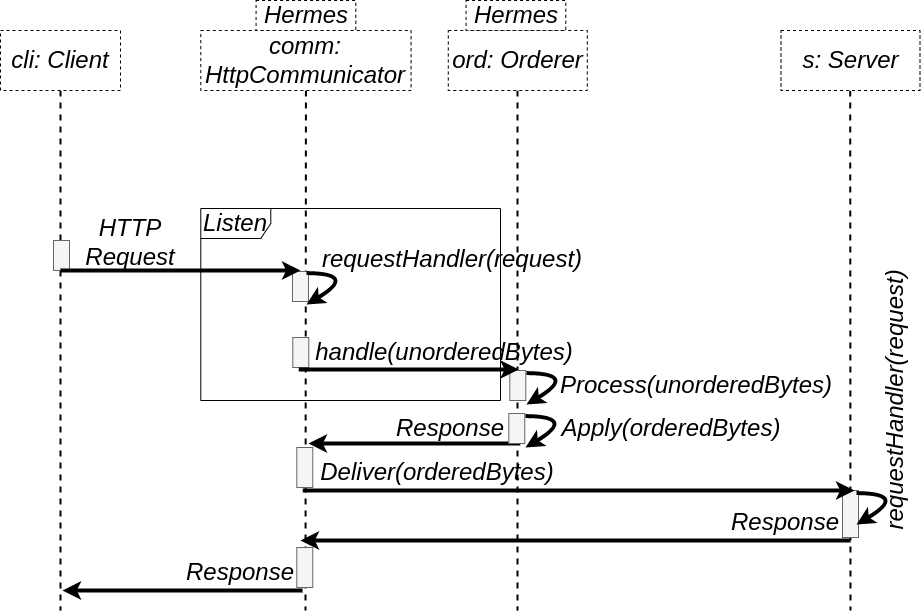
\includegraphics[width=\linewidth]{figures/deliver-listen-logic.drawio.png}
{\flushleft Fonte - Própria}
\label{fig:deliver-listen-logic}
\end{figure}

A Figura \ref{fig:deliver-listen-logic} mostra um diagrama do fluxo de informação passando pelos métodos \textit{Listen} e \textit{Deliver}. Uma vez que uma requisição HTTP qualquer é interceptada pelo Hermes, o evento Listen irá capturar essa requisição e transformar a requisição HTTP em \textit{bytes} e passar ao \textit{handler}. O \textit{handler} irá levar a informação em arranjo de bytes para ser ordenador pelo algoritmo de ordenação. Uma vez que o arranjo de \textit{bytes} está ordenado ele entra no método \textit{Deliver} e portanto eles já estão garantidamente ordenados.


\subsection{Experimentação}

Esta sessão trata como foram realizados as experimentações e, além disso, são mostrados as configurações para os experimentos.

\begin{figure}[htb!]
\centering
\caption{Representações das configurações sem replicação (A) e com ordenação respectivamente (B)}
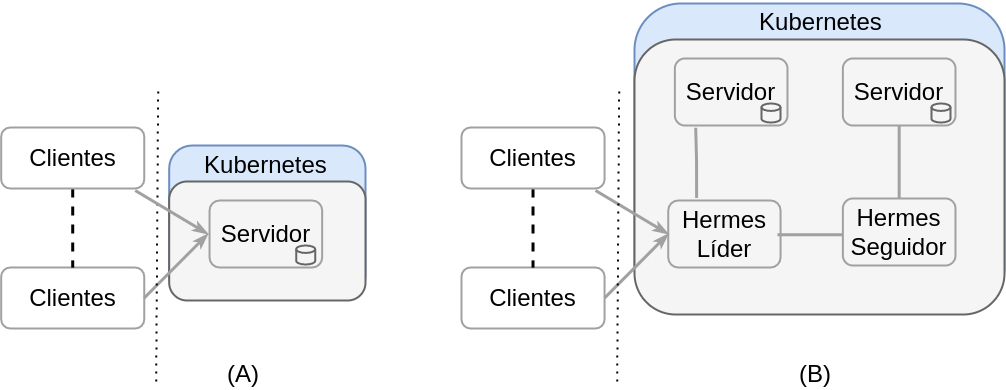
\includegraphics[width=\linewidth]{figures/confiuracoes-kubernetes.drawio.png}
{\flushleft Fonte - Adaptado de \textcite{renan2021hermes}}
\label{fig:arquitetura-cluster-ordenadores}
\end{figure}

\textit{Replicação com ordenação pelo interceptador:} A combinação para este cenário utiliza instâncias para gerador de carga, o servidor de armazenamento de \textit{logs}
sem consenso e o interceptador Hermes. Este cenário será utilizado para avaliar o custo médio de vazão de requisições HTTP.

\pagebreak

A Figura \ref{fig:arquitetura-cluster-ordenadores} (lado A) mostra a configuração do servidor sem replicação e a Figura \ref{fig:arquitetura-cluster-ordenadores} (lado B) mostra a configuração do servidor com replicação. Notar que o ordenador de mensagens fica à frente de cada réplica. Estas configurações foram usadas para os experimentos em ambiente real com implantação de orquestrador de contêineres. Este trabalho inclui duas aplicações que foram implementadas para os experimentos o \textit{HttpLogServer} e o \textit{HttpLogClient}, que serão explicadas a seguir. A aplicação \textit{HttpLogServer} tem basicamente 2 funções:

\begin{itemize}
\item Adicionar no fim de um arquivo (\textit{/tmp/logs/operations.txt}) as inserções via requisição POST.
\item Iterar sobre as linhas do arquivo \textit{/tmp/logs/operations.txt} e retornar a linha requerida via requisição GET.
\end{itemize}

Foi necessário implementar um servidor \gls{HTTP} customizado, usando as bibliotecas \textit{http.server} e \textit{sockethandler} para haver liberdade em registrar a contagem de requisições atendidas pelo servidor.

\subsection{Desenvolvimento}

O desenvolvimento do protocolo \gls{HTTP} foi feito em linguagem Go. O código atual do trabalho pode ser encontrado no Capítulo \ref{cap:conclusao}. Caso seja necessário alterar o código fonte, é recomendado alterar o nome do pacote Go, de `tonussi/hermes` para `xyz/hermes`. Também é recomendado criar um repositório no Github como `xyz/hermes`. Depois de alterar o nome do pacote Go, remova os arquivos \textit{go.mod} e \textit{go.sum} e execute as linhas a seguir:

\begin{verbatim}
go mod init github.com/xyz/hermes
go mod tidy
go get -u all
\end{verbatim}

\subsection{Detalhes de construção dos contêineres}

Para desenvolver no código se recomenda instalar o Docker Compose (define e executa contêineres Docker), o Docker (criador de imagens e contêineres de aplicação), Vscode (editor de código), \textit{make} (programa para executar comandos no Makefile), Makefile é um descritor de comandos úteis a serem executados pelo programa make. Uma vez instalados é possível apenas executar \textit{make build\_debug\_hermes}, para gerar imagem de contêiner para um Hermes com depurador Delve embutido. Fazendo isto deve ser possível acionar o modo Executar e Depurar selecionando a opção \textit{Debug Hermes (Attach)}, pois há um arquivo \textit{.vscode/launch.json} que integra o Delve com o Docker.

O Depurador indicará qual linha de código está sendo depurada. Como o Go é compilado, não é recomendado alterar o código e re-depurar imediatamente, então basta recompilar o código. O depurador Delve, ajuda a enxergar como o código está se comportando e, quais informações estão passado pelas funções.

Algumas notas importantes são, o arquivo Docker Compose irá gerar: um volume de dados para o BoltDB\footnote{BoltDB: \url{https://github.com/boltdb/bolt}} e um banco de dado usado internamente pelo Raft (interno ao Hermes). Por padrão o Hermes irá escutar o endereço \gls{IP}:8000 e enviar para o endereço \gls{IP}:8001.

O servidor da aplicação alvo poderá escutar no endereço \gls{IP}:8001. A menos que seja necessário alterar os endereços e portas, no caso se o servidor da aplicação precisar escutar outra porta, basta alterar o endereço de envio do Hermes via parâmetros.

